\appendix
\renewcommand{\appendixtocname}{Appendix}
\renewcommand{\appendixpagename}{\appendixtocname}
\addappheadtotoc
\setboolean{@twoside}{false}
\appendixpage

\chapter{\ac{DQN} Policy Replay Samples}\label{app:replay}

\noindent These three frames are consecutive steps from Episode 2 of a trained \ac{DQN} policy replay, captured with the replay viewer tool. Each frame substitutes the current state into the thesis reward function $r = w_k\,\Delta K + w_e E - w_f F - w_b B - w_c C$ to illustrate the policy's real-time responsiveness across three decisions.


\noindent Across these steps, the policy transitions from \textbf{scaffold} to \textbf{harder problem} as the learner's knowledge level increases, and then to \textbf{explanation} when confusion rises. The sequence reflects the behaviour of the trained \ac{DQN} policy as it reacts to changes in the observed student state.

\begin{figure}[h]
\centering
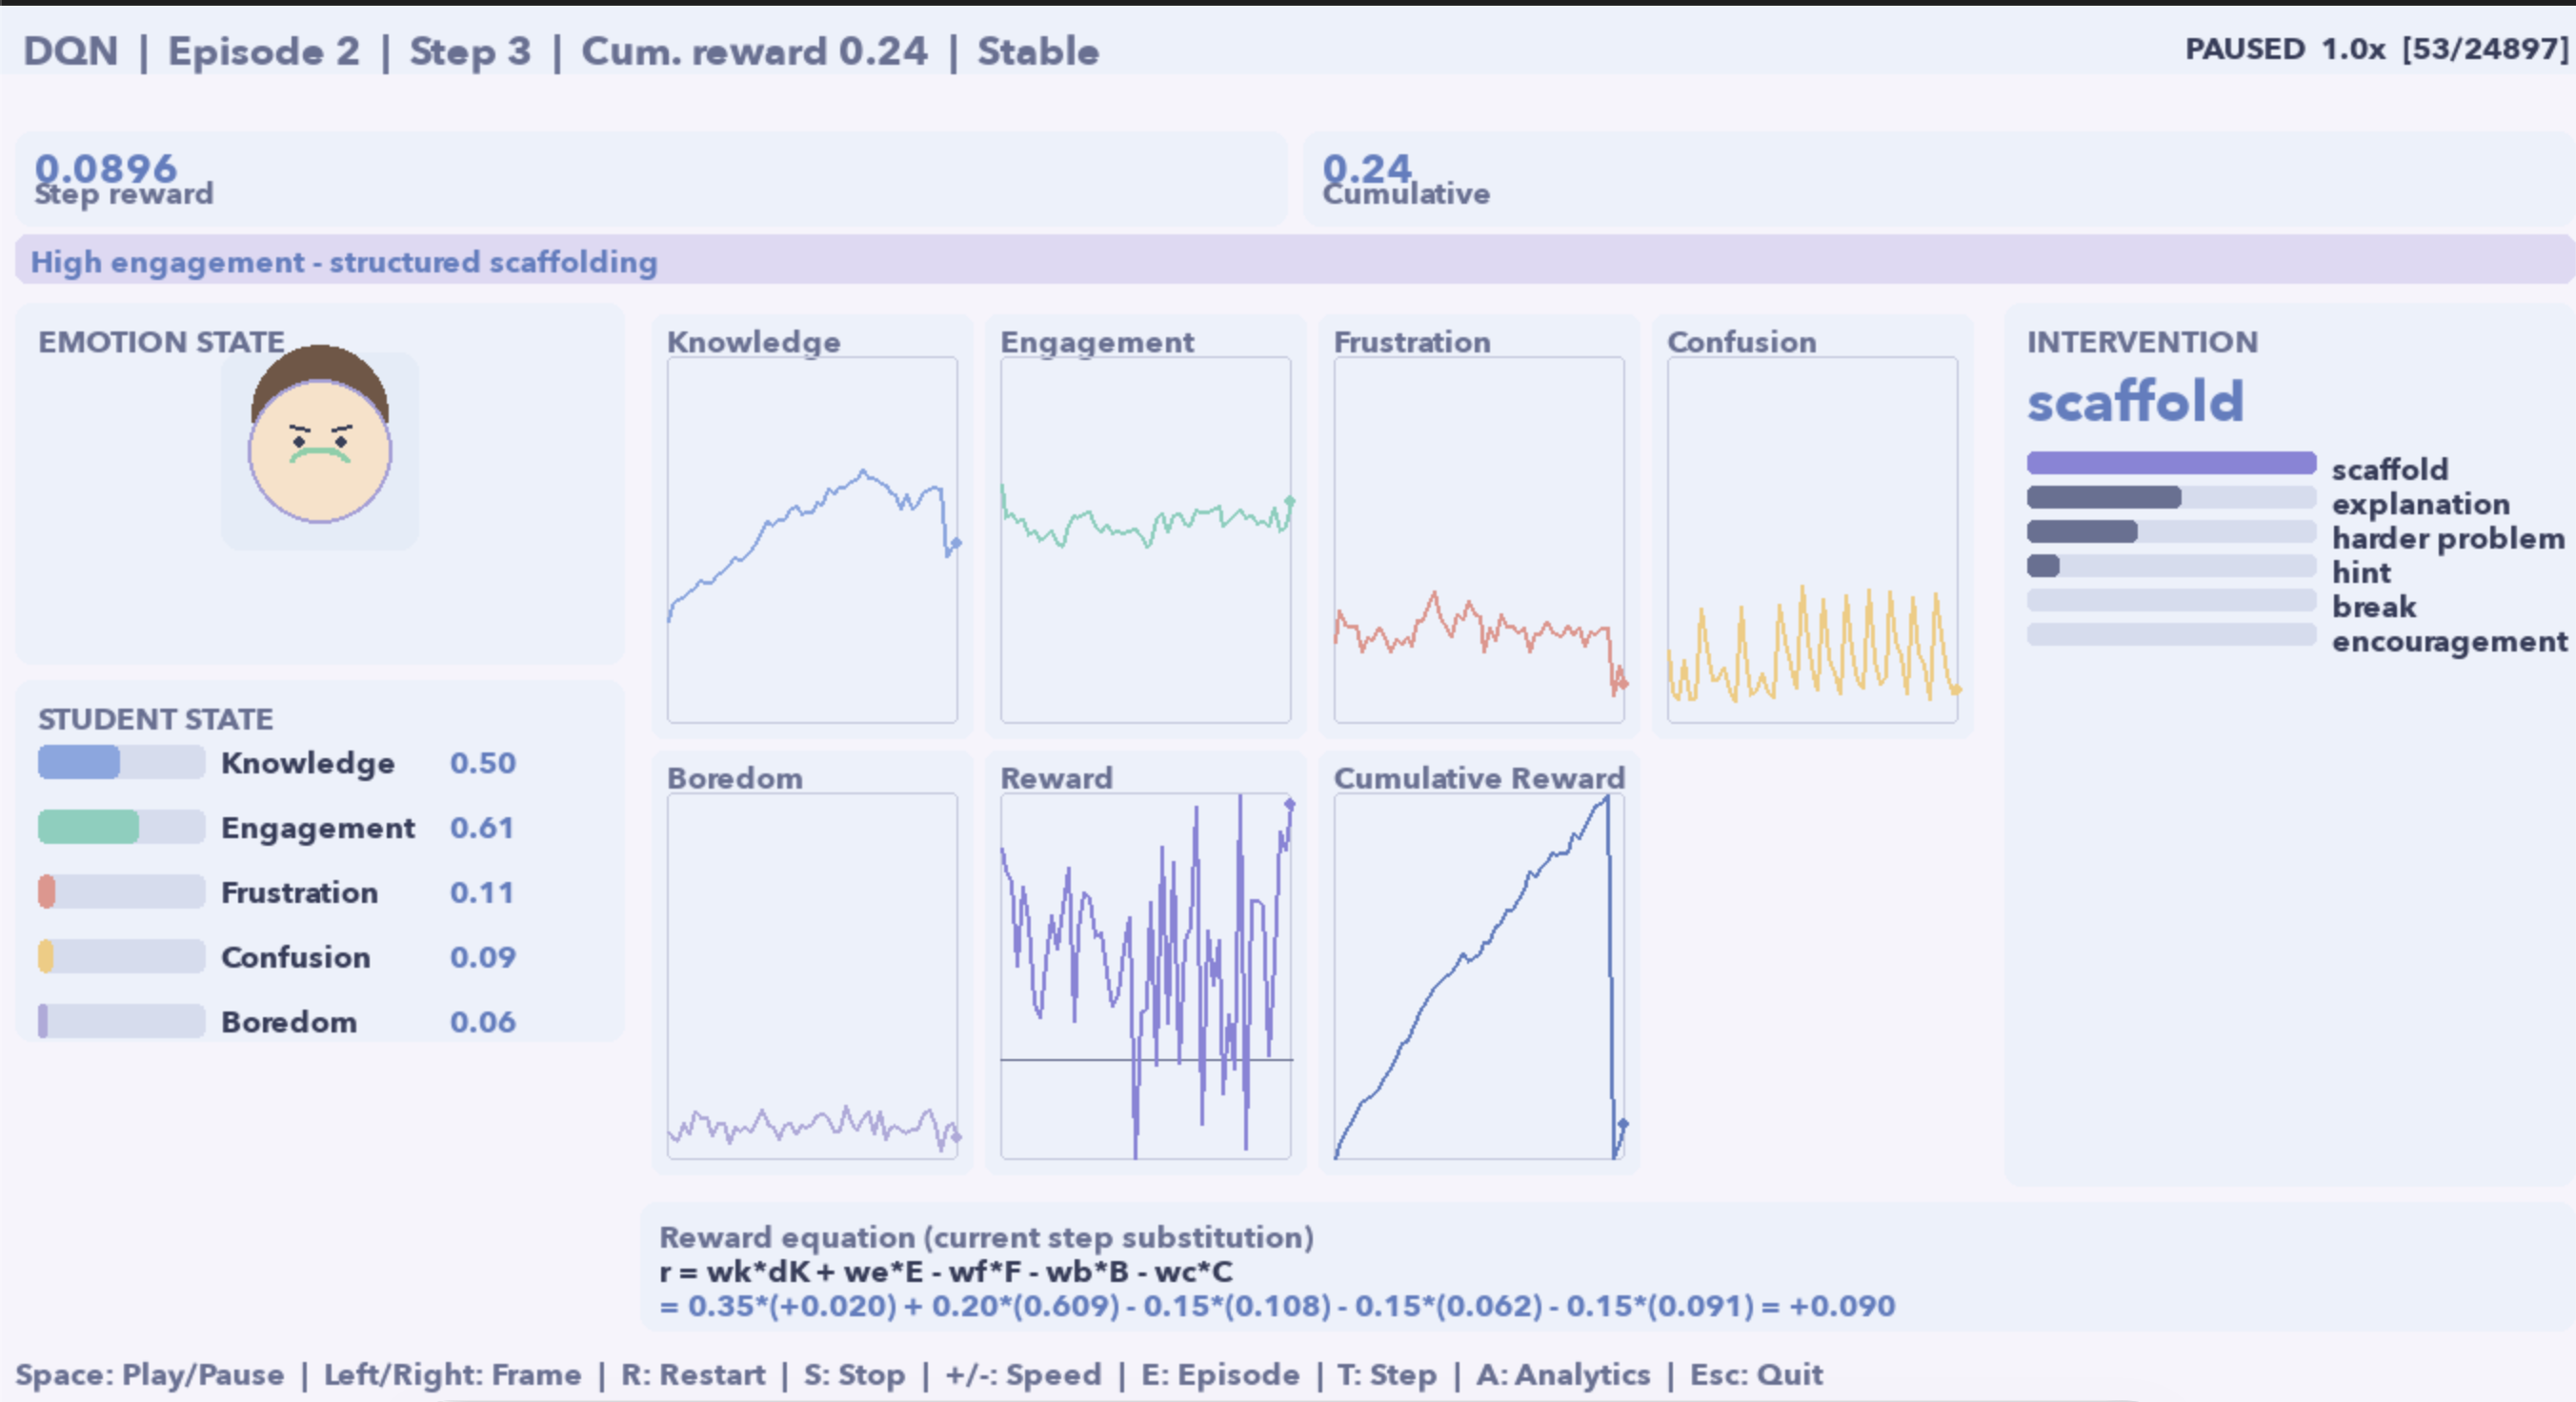
\includegraphics[width=\textwidth]{Figures/one.png}
\caption{Episode 2, Step 3, cumulative reward $0.24$, with student state Knowledge $0.50$, Engagement $0.61$, Frustration $0.11$, Confusion $0.09$, Boredom $0.06$. The policy selected \textbf{scaffold}, a flow-consistent choice that structures a high-engagement learner without raising difficulty, yielding a step reward of $0.0896$.}
\label{fig:replay_step3}
\end{figure}

\begin{figure}[h]
\centering
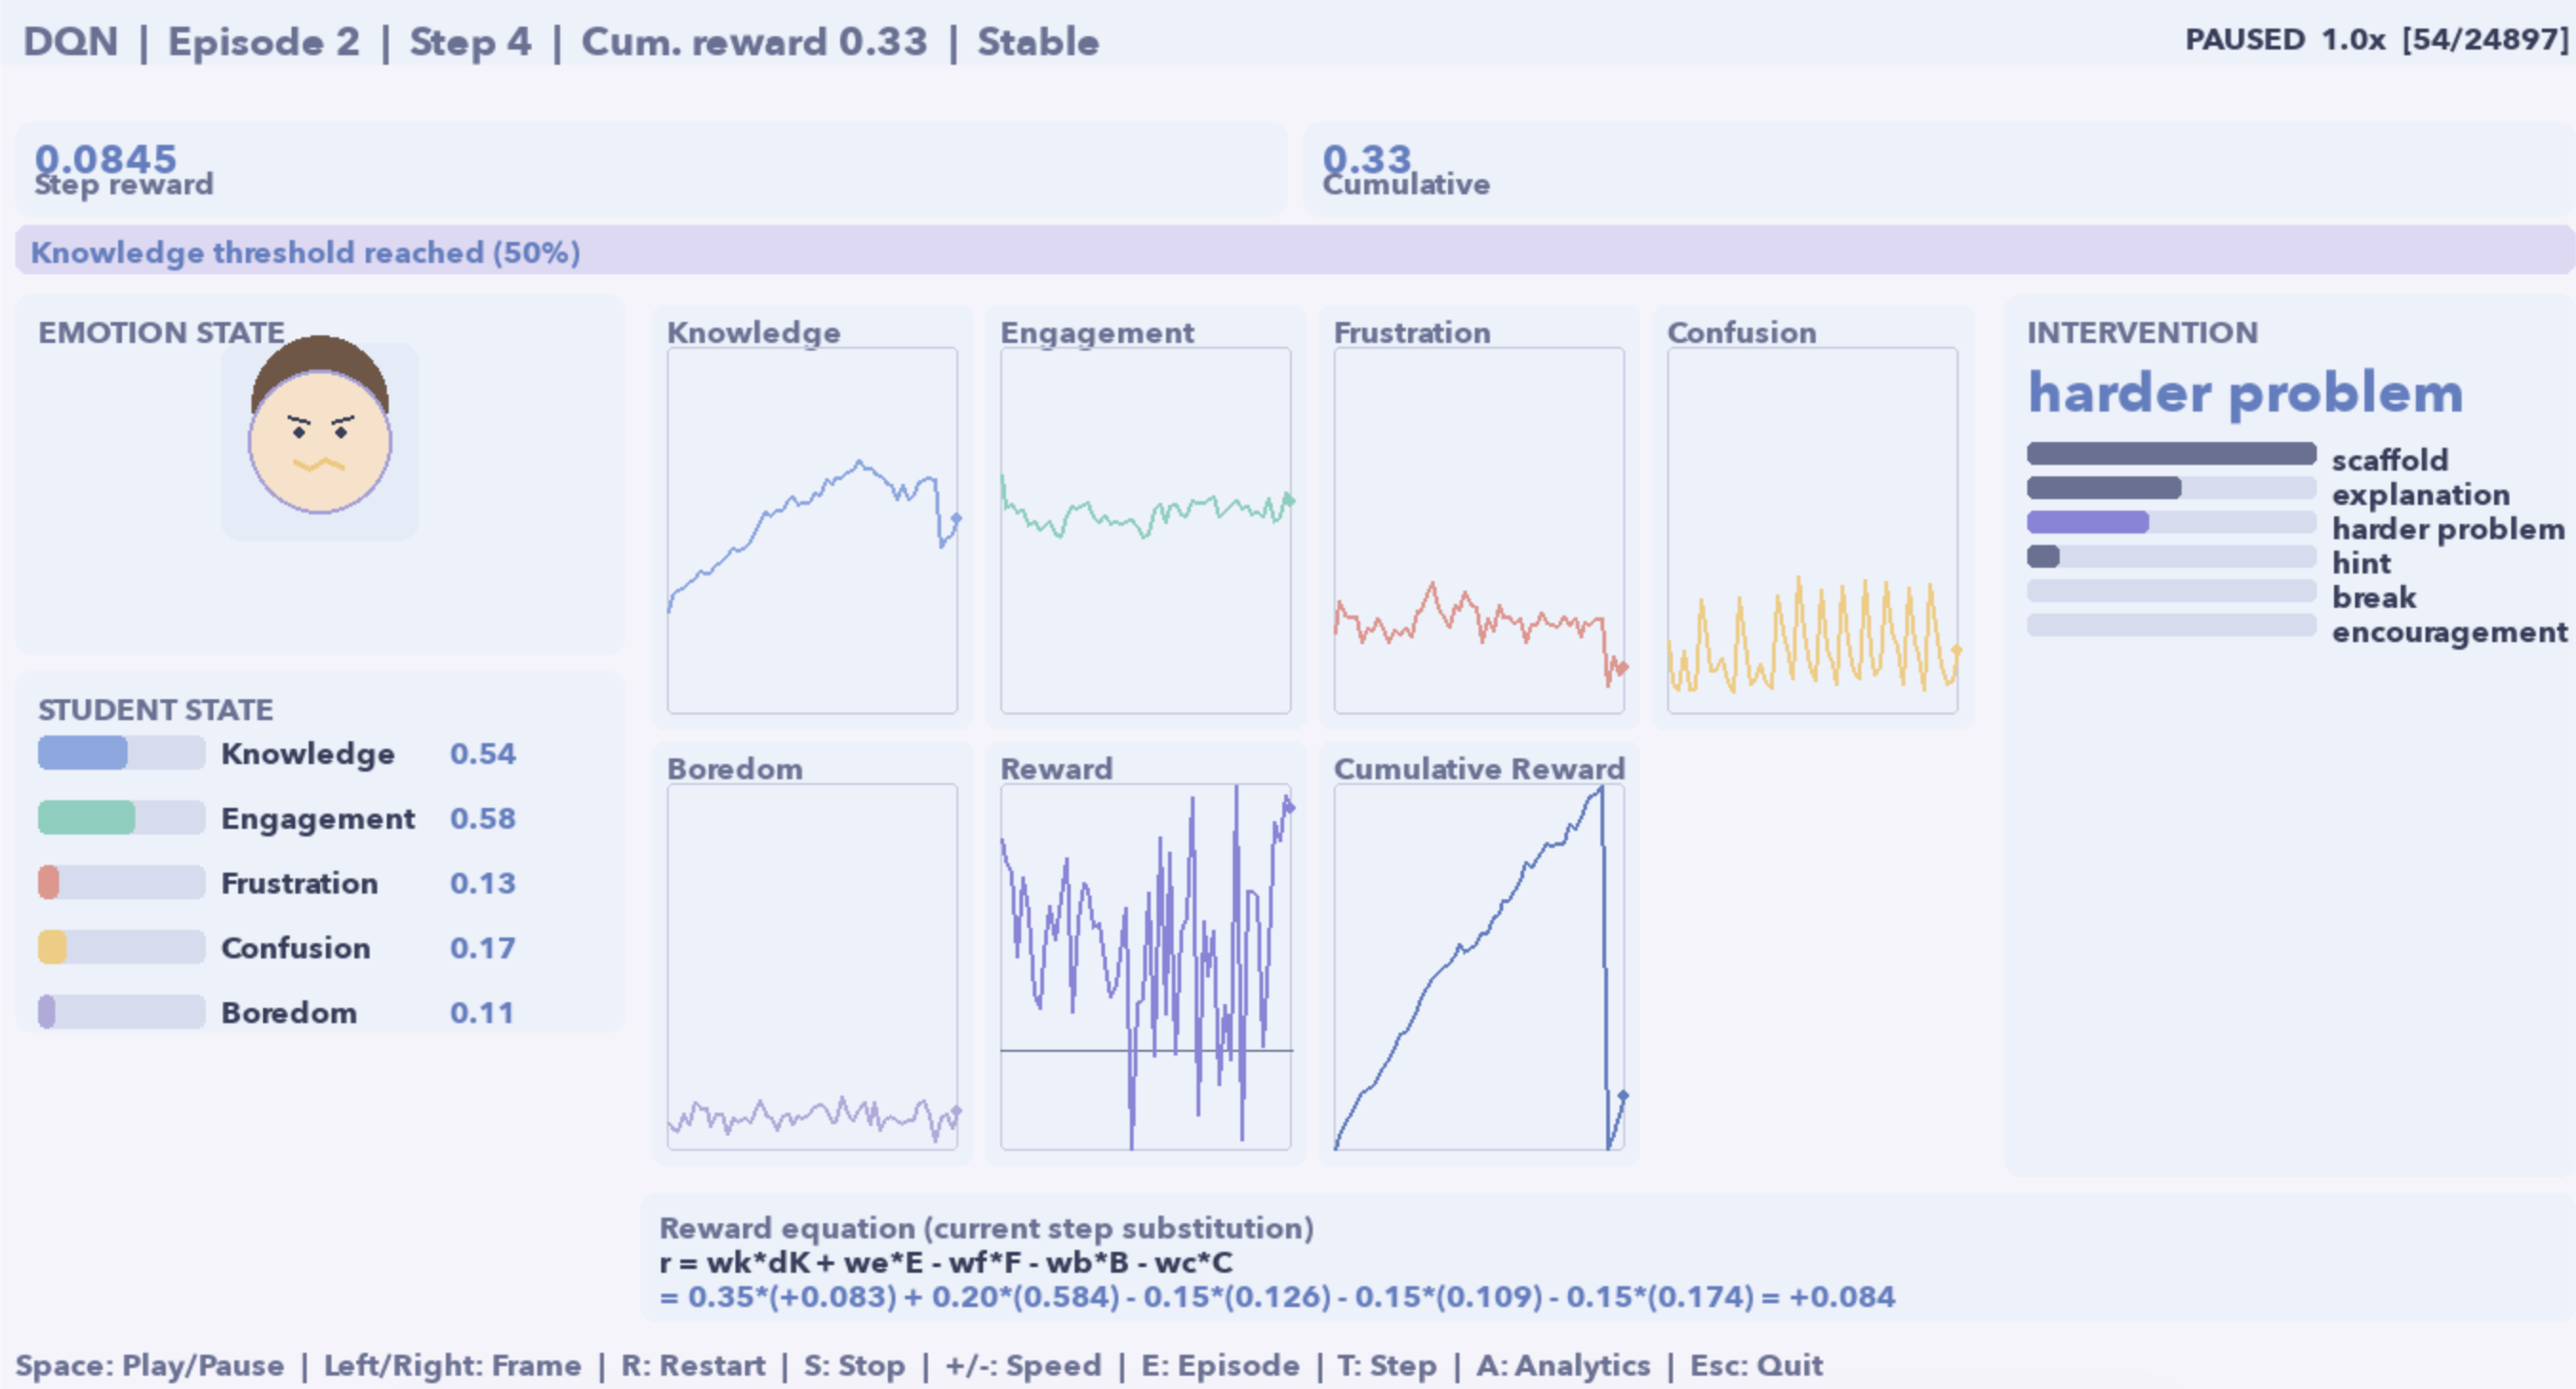
\includegraphics[width=\textwidth]{Figures/two.png}
\caption{Episode 2, Step 4, cumulative reward $0.33$, with student state Knowledge $0.54$, Engagement $0.58$, Frustration $0.13$, Confusion $0.17$, Boredom $0.11$. The policy selected \textbf{harder problem} as the learner's knowledge level increased to approximately $0.54$, resulting in a rise in confusion to $0.17$ following the increase in task difficulty, with a step reward of $0.0845$.}
\label{fig:replay_step4}
\end{figure}



\begin{figure}[h]
\centering
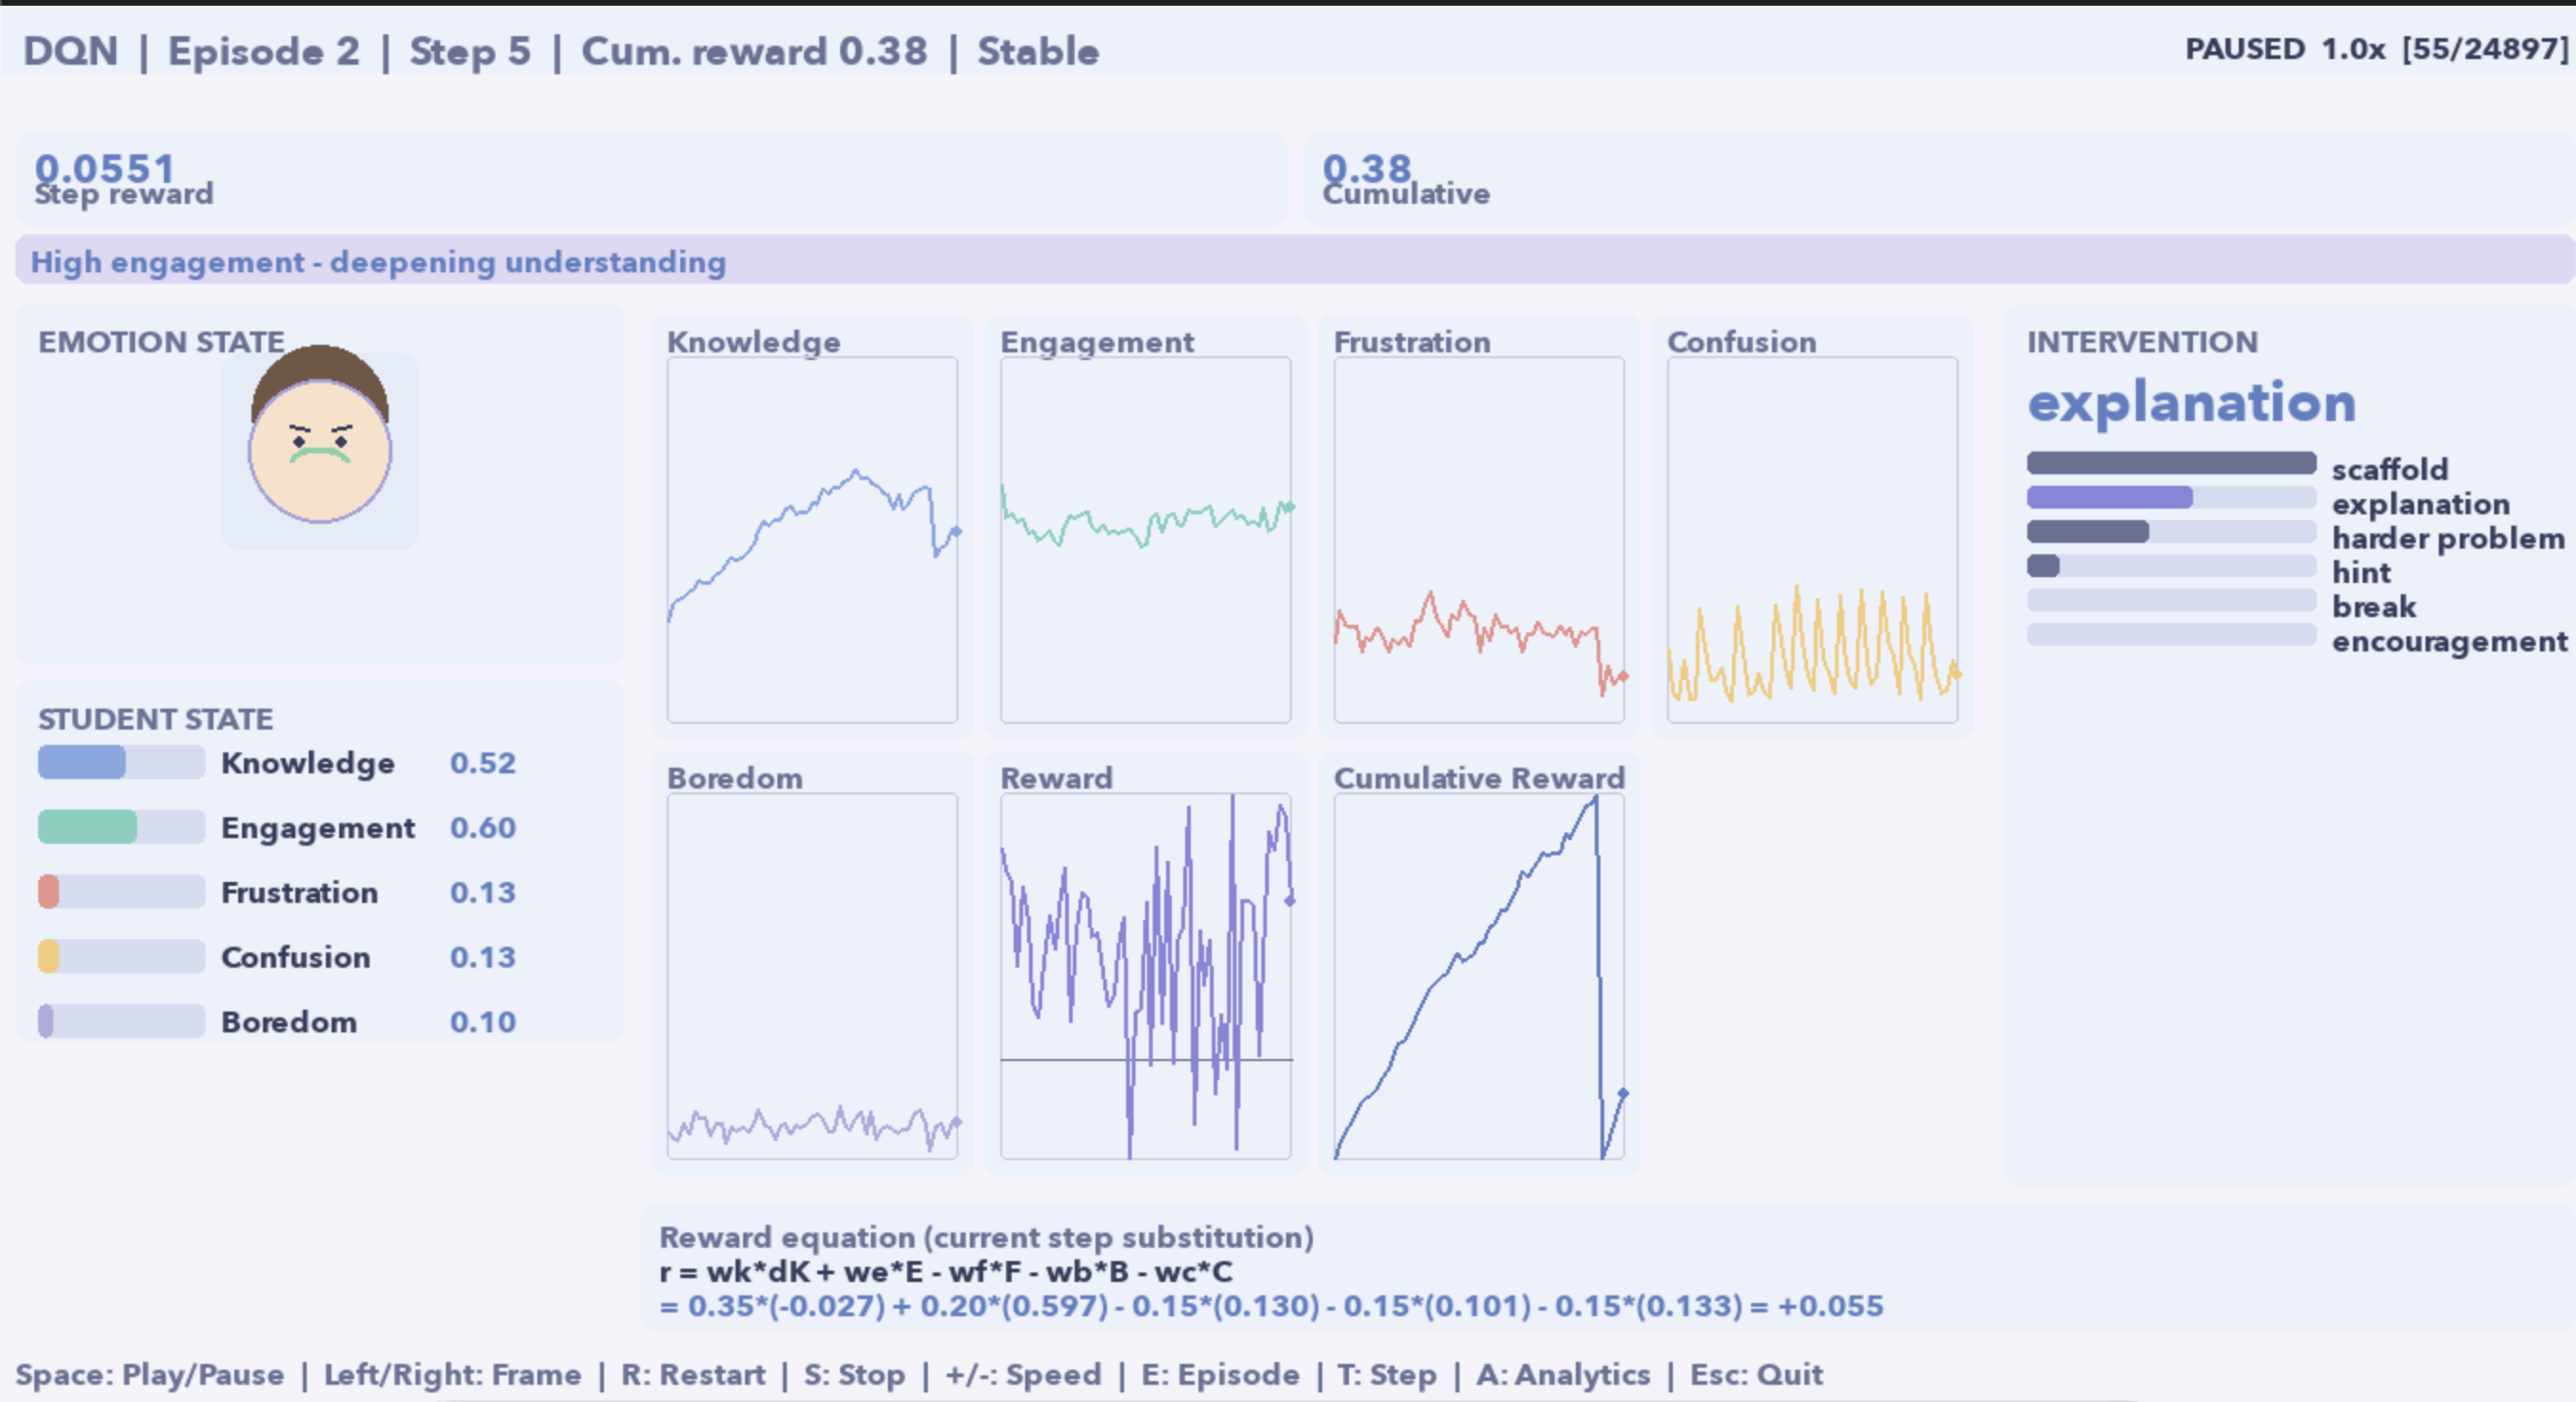
\includegraphics[width=\textwidth]{Figures/three.png}
\caption{Episode 2, Step 5, cumulative reward $0.38$, with student state Knowledge $0.52$, Engagement $0.60$, Frustration $0.13$, Confusion $0.13$, Boredom $0.10$. In response to the prior confusion rise, the policy selected \textbf{explanation}, which lowered confusion to $0.13$ while engagement stayed high, yielding a step reward of $0.0551$.}
\label{fig:replay_step5}
\end{figure}


% Add all other equations or figures or as you wish here...